\documentclass{article}

\usepackage[utf8]{inputenc}
\usepackage[T1]{fontenc}
\usepackage[portuguese]{babel}
\usepackage{amsmath}
\usepackage{amssymb}
\usepackage{bbm}
\usepackage{circuitikz}
\usepackage{pgfplots}
\usepackage{float}

\newcommand\tab[1][0.6cm]{\hspace*{#1}}

\title{Lei de Ohm e curva característica do diodo}
\author{
    Eduardo Parducci - 170272
    \and
    Lucas Koiti Geminiani Tamanaha - 182579
    \and
    Rodrigo Seiji Piubeli Hirao - 186837
    \and
    Tanus Vaz Szabo - 187308
}
\date{\today}

\begin{document}
    \maketitle
\newpage
\tableofcontents
\newpage
    \section{Material Utilizado}
        \begin{itemize}
    \item [1] Bobina de Helmholtz 
        \begin{itemize}
             \item [n] 140 espiras
             \item [D] 22,3cm
             \item [d] 20,2cm
             \item [l] 1,13cm
             \item [L] 10,26cm
        \end{itemize}
    \item [1] Bússola
    \item [1] Ímã permanente cilíndrico 
        \begin{itemize}
             \item [D] 0,6cm
             \item [l] 2,53cm
             \item [m] 5,1616g
        \end{itemize}
    \item [1] Multímetro
    \item [1] Resistor de potência
    \item [1] Fonte de alimentação
    \item [1] Cronômetro
    \item [6] Fios de ligação
\end{itemize}
    \section{Procedimento}
        \subsection{Determinar resistência $R_{x}$ utilizando a ponte de Wheatstone}
            \tab Com o uso do multímetro na escala $\Omega$, checar o valor dos resistores nominais de
            $68\Omega$ e $100\Omega$ anotando os valores e respectivos erros comparando-os com o nominal.
            \par
            Determinar o valor da tensão para a montagem do circuito 1 de forma que $R_{v}$ varie entre $10\Omega$ e $60\Omega$
            fazendo com que potência dissipada em $R_{p}=100\Omega$ não ultrapasse $1,5W$.
            \par
            Montar o circuito 1 (Ponte de Wheatstone) e realizar 20 medições da tensão (multímetro na escala $V\backsimeq$ )
            variando $R_{v}$ entre $10\Omega$ e $60\Omega$. Colocar os valores e seus respectivos erros em uma tabela
            $R_{v}\pm\Delta R_{v}$ e $V\pm\Delta V$.\newline
            \textbf{Obs:}Diminuir a variação $\Delta R_{v}=0,1\Omega$ quando os valores da tensão estiverem próximos de zero a fim de obter um
            gráfico mais consistente.
        \subsection{Determinar os coeficientes de fabricação do termistor}
            \tab Anotar o número do termistor utilizado e montar o circuito 2 mantendo $R_{p}=100\Omega$.
            \par
            Colocar água e o aquecedor no Béquer de forma que a resistência do Aquecedor fique totalmente submersa na água.
            \par
            Ligar o Aquecedor e medir a temperatura da água, até atingir $T_{max}=333K$, desligar o aquecedor e realizar 30 medidas
            da tensão até atingir $T_{min}=303K$ obtendo uma leitura a cada $\Delta T = 1K$ colocando os valores numa tabela $T\pm\Delta T$
            e $V\pm\Delta V$.
    \newpage
\section{Anexo}
    \listoffigures
    \newpage
    
    \subsection{Circuitos Utilizados}
        \begin{figure} [H]
    \def\x{6}
    \def\y{6}

    \def\dx{3}
    \def\dy{3}

    \begin{circuitikz}

        \draw (0,0) to [battery=$12V$](0, \y) to (\x, \y)
        to [R=100$\Omega$, -] (\x-\dx,\y-\dy)
        to [R=100$\Omega$, -*] (\x,\y-2*\dy);

        \draw (\x,\y)
        to [R=68$\Omega$, -*] (\x+\dx, \y-\dy)
        to [R, l_=$R_{v}$, -*] (\x,\y-2*\dy)
        to (\x, 0) to (0,0);

        % Voltimetro
        \draw (\x-\dx, \y-\dy) to [voltmeter] (\x+\dx, \y-\dy);
    \end{circuitikz}

    \caption{Circuito com Ponte de Wheatstone}
    \label{fig:circuitW}
\end{figure}

    \subsection{Gráficos Produzidos}
        \subsubsection{Resistor ixU}
\begin{figure} [H] 
    \centering
    \pgfplotstableset{
        columns/x/.style={
            column name={$U[V]$},
        },
        columns/y/.style={
            column name={$i[mA]$},
        },
        columns/ex/.style={
            column name={$\Delta U[V]$},
        },
        columns/ey/.style={
            column name={$\Delta i[mA]$},
        },
    }
    \pgfplotstableread{data/resistor.dat}\loadedtable
    \pgfplotstabletypeset{\loadedtable}
    \caption{Tabela de dados da corrente adquirida ao aumentar tensão em resistor}
    \label{fig:tableR}
\end{figure}

\begin{figure} [H] 
    \centering
    \begin{tikzpicture}
        \begin{axis}[
            width=10cm,
            xlabel={$U[V]$},
            ylabel={$i[A]$},
            xlabel style={below right},
            ylabel style={above left},
            ]
            \addplot [color=cyan, mark=o, smooth, ultra thick]
                plot [error bars/.cd, y dir = both, y explicit]
                table[x =x, y =y]{data/resistor.dat};
        \end{axis}
    \end{tikzpicture}
    \caption{Gráfico da corrente adquirida ao aumentar tensão em resistor}
    \label{fig:graphR}
\end{figure}

\subsubsection{Diodo ixU}
\begin{figure} [H] 
    \centering
    \pgfplotstableset{
        columns/x/.style={
            column name={$U[V]$},
        },
        columns/y/.style={
            column name={$i[mA]$},
        },
        columns/ex/.style={
            column name={$\Delta U[V]$},
        },
        columns/ey/.style={
            column name={$\Delta i[mA]$},
        },
    }
    \pgfplotstableread{data/diodo.dat}\loadedtable
    \pgfplotstabletypeset{\loadedtable}
    \caption{Gráfico da corrente adquirida ao aumentar tensão em diodo}
    \label{fig:tableD}
\end{figure}

\begin{figure} [H] 
    \centering
    \begin{tikzpicture}
        \begin{axis}[
            width=10cm,
            xmode=log,
            xlabel={$U[V]$},
            ylabel={$i[mA]$},
            xlabel style={below right},
            ylabel style={above left},
            ]
            \addplot [color=cyan, mark=o, smooth, ultra thick]
                plot [error bars/.cd, y dir = both, y explicit]
                table[x =x, y =y, x error=ex, y error=ey]{data/diodo.dat};
        \end{axis}
    \end{tikzpicture}
    \caption{Gráfico da corrente adquirida ao aumentar tensão em diodo}
    \label{fig:graphD}
\end{figure}


\subsubsection{Diodo RxU}
\begin{figure} [H] 
    \centering
    \pgfplotstableset{
        columns/x/.style={
            column name={$U[V]$},
        },
        columns/y/.style={
            column name={$R[\Omega]$},
        },
        columns/ex/.style={
            column name={$\Delta U[V]$},
        },
        columns/ey/.style={
            column name={$\Delta R[\Omega]$},
        },
    }
    \pgfplotstableread{data/diodo2.dat}\loadedtable
    \pgfplotstabletypeset{\loadedtable}
    \caption{Gráfico da resitência adquirida ao aumentar tensão em diodo}
    \label{fig:tableD2}
\end{figure}

\begin{figure} [H] 
    \centering
    \begin{tikzpicture}
        \begin{axis}[
            width=10cm,
            xmode=log,
            xlabel={$U[V]$},
            ylabel={$R[\Omega]$},
            xlabel style={below right},
            ylabel style={above left},
            ]
            \addplot [color=cyan, mark=o, smooth, ultra thick]
                plot [error bars/.cd, y dir = both, y explicit]
                table[x =x, y =y, x error=ex, y error=ey]{data/diodo2.dat};
        \end{axis}
    \end{tikzpicture}
    \caption{Gráfico da resistência adquirida ao aumentar tensão em diodo}
    \label{fig:graphD2}
\end{figure}


\begin{figure} [H] 
    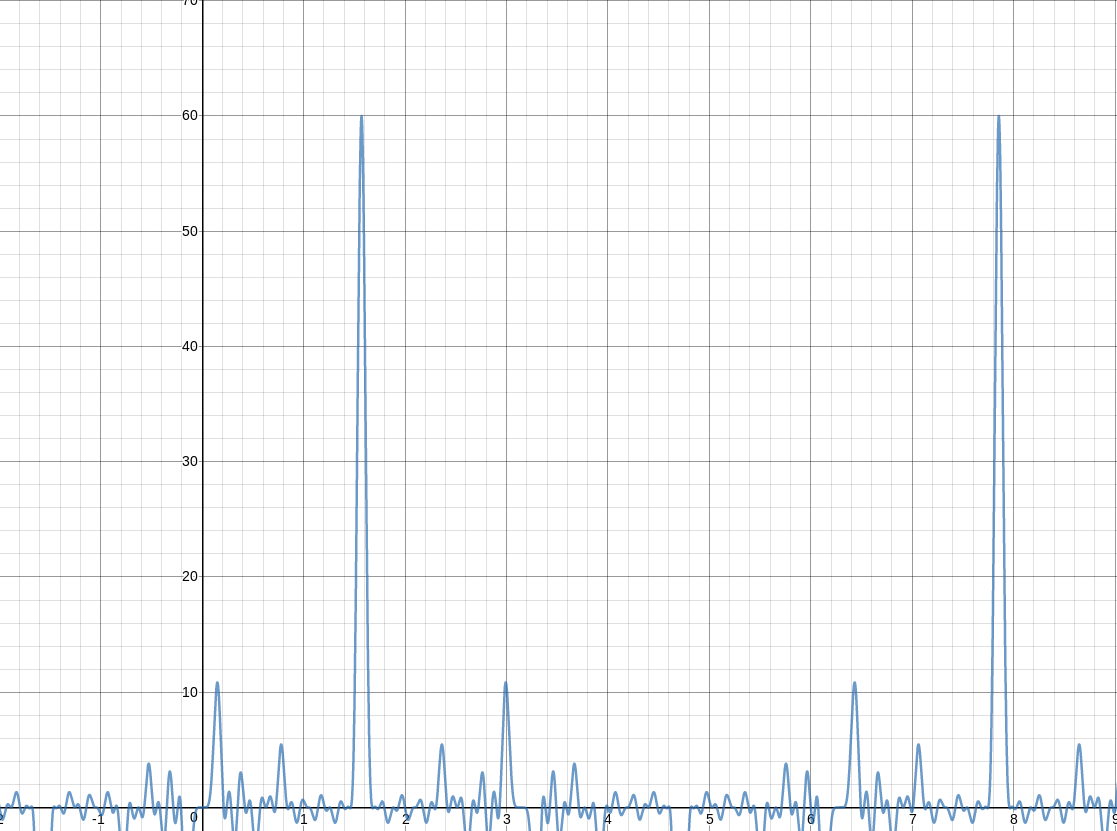
\includegraphics{graph}
    \caption{Gráfico do MMQ}
    \label{fig:graphMMQ}
\end{figure}
\end{document}